\section{Frameworks measurements}

We describe in this section the results obtained with the extension framework described in the section \ref{sec:extension} and with the devices framework described in the section \ref{sec:external}.
In the same way as with the reference value, the results are divided by boards.
The measurements made with the RE-Mote boards are first given, then the one made with Z1 board.
The Contiki measurements are displayed side-by-side with the RIOT OS one.

\subsection{Extension framework measurements}

\subsubsection{RE-Mote measurements}
On the RE-Mote board, the extension framework outputs an average context switching time of $31.6162\mu s$ on Contiki and $17 \mu s$ on RIOT OS.
The table \ref{tab:extension-framework-remote} shows the measurement for Contiki and RIOT OS for the RE-Mote board.

With Contiki, we had extreme values from $0\mu s$ to $457.7636\mu s$.
In the other hand, with RIOT, all of the 1000 measurements were equal to $17\mu s$.
The difference with the reference is value is $13.1112 \mu s$ with Contiki and $4.374 \mu s$ with RIOT.
Both measurements were above the real context switching time given by the reference value.

\begin{table}[!ht]
  \centering
  \begin{tabular}{l|c|c}
                & Contiki  & RIOT \\ \hline
  Mean ($\mu$s) & 31.6162  & 17      \\
  Min  ($\mu$s) & 0        & 17      \\
  Max  ($\mu$s) & 457.7636 & 17     
  \end{tabular}
  \caption{extension approach measurements for Contiki and RIOT on the RE-Mote board}
  \label{tab:extension-framework-remote}
  \end{table}

% \begin{figure}[!ht]
%   \begin{minipage}{.45\textwidth}
%       \centering
%       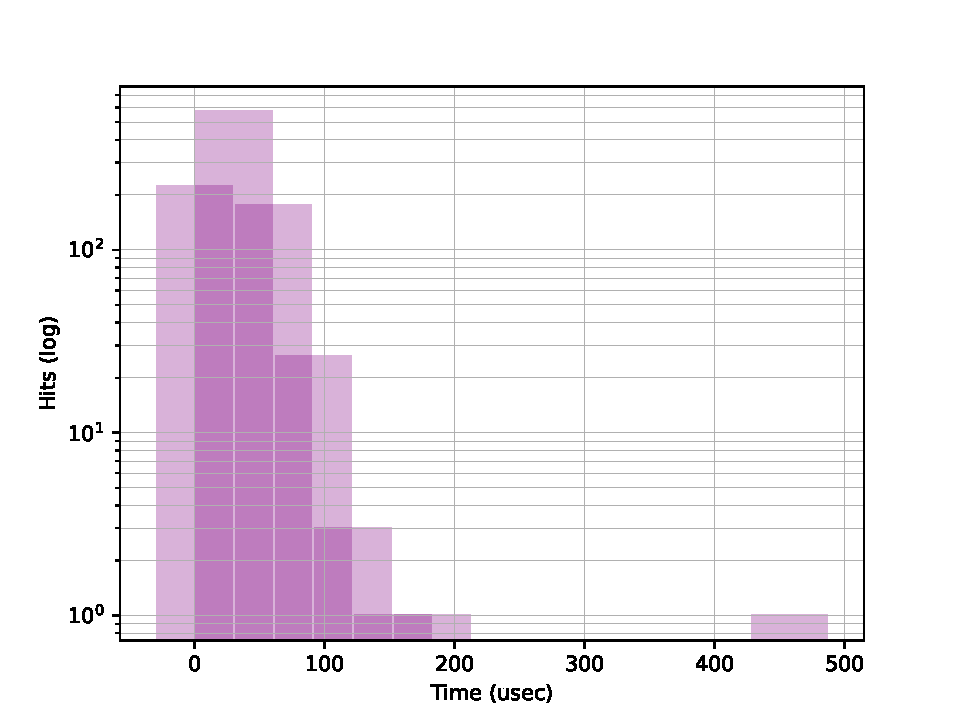
\includegraphics[scale=.4]{assets/extension-framework-contiki-remote.pdf}
%       \caption{Extension framework distribution with Contiki on RE-Mote\label{fig:extension-framework-contiki-remote}}
%   \end{minipage}\hfill
%   \begin{minipage}{.45\textwidth}        
%       \centering
%       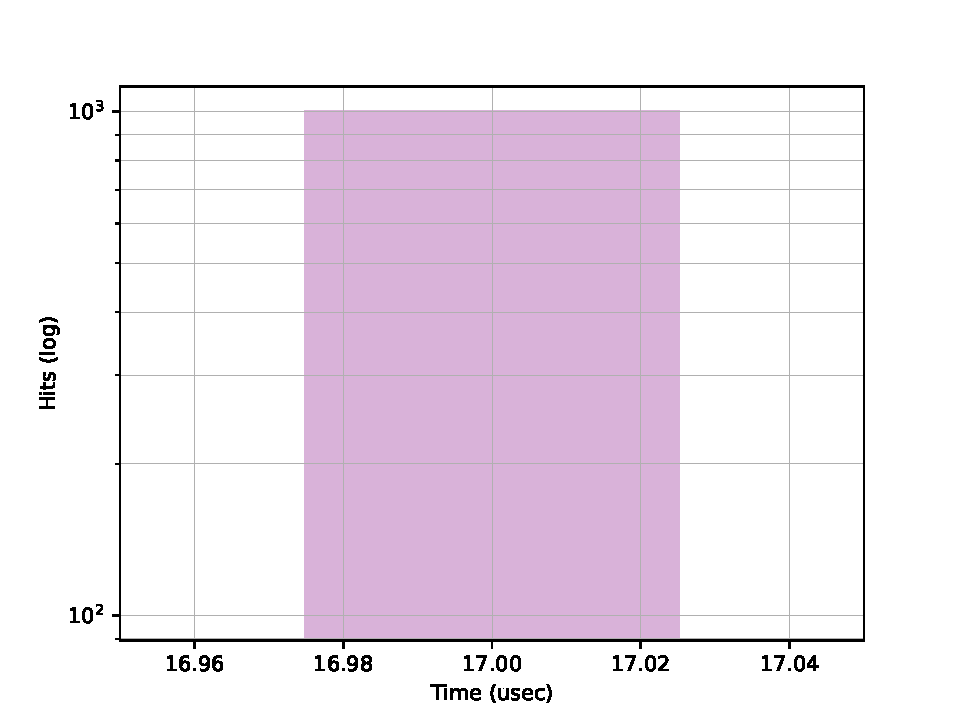
\includegraphics[scale=.4]{assets/extension-framework-riot-remote.pdf}
%       \caption{Extension framework distribution with RIOT on RE-Mote\label{fig:extension-framework-riot-remote}}
%   \end{minipage}
% \end{figure}

\subsubsection{Z1 measurements}
On the Class-1 Z1 board, the extension framework gave an average context switching of $90.5761\mu s$ with Contiki and $40.252\mu $s with RIOT OS.
The table \ref{tab:extension-framework-z1} shows the measurement for Contiki and RIOT OS for the Z1 board.

Once again, on Contiki, our values were largely distributed between $30.5175\mu s$ and $976.5625\mu s$.
With RIOT, most of the values where equal to $40 \mu s$.
The difference with the reference is value is $35.4991 \mu s$ with Contiki and $12.553 \mu s$ with RIOT.
Both measurements were above the real context switching time given by the reference value.

\begin{table}[!ht]
  \centering
  \begin{tabular}{l|c|c}
                & Contiki  & RIOT \\ \hline
  Mean ($\mu$s) & 90.5761  & 40.252      \\
  Min  ($\mu$s) & 30.5175  & 40      \\
  Max  ($\mu$s) & 976.5625 & 41     
  \end{tabular}
  \caption{extension approach measurements for Contiki and RIOT on the Z1 board}
  \label{tab:extension-framework-z1}
  \end{table}

% \begin{figure}[!ht]
%   \begin{minipage}{.45\textwidth}
%       \centering
%       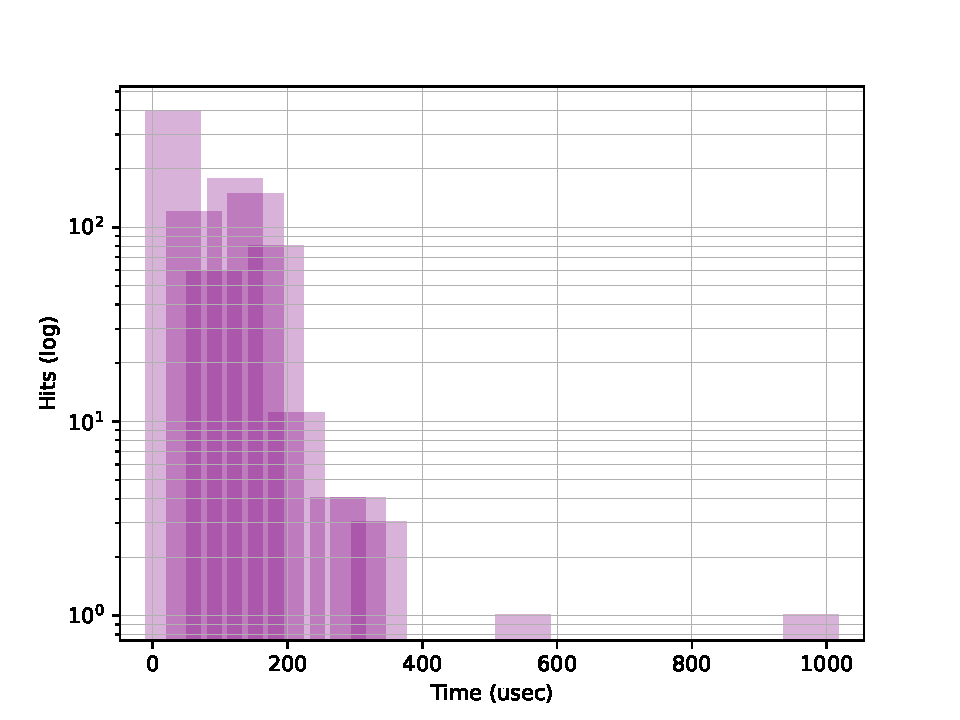
\includegraphics[scale=.4]{assets/extension-framework-contiki-z1.pdf}
%       \caption{Extension framework distribution with Contiki on Z1\label{fig:extension-framework-contiki-z1}}
%   \end{minipage}\hfill
%   \begin{minipage}{.45\textwidth}        
%       \centering
%       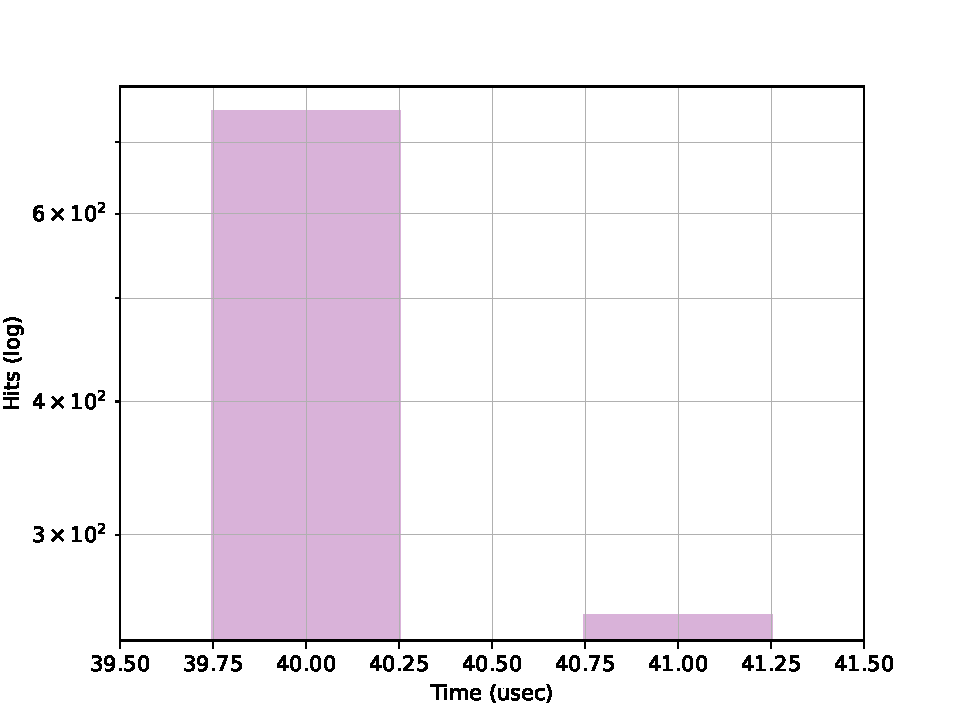
\includegraphics[scale=.4]{assets/extension-framework-riot-z1.pdf}
%       \caption{Extension framework distribution with RIOT on Z1\label{fig:extension-framework-riot-z1}}
%   \end{minipage}
% \end{figure}

% \subsection{Discussion}

% To discuss the results, we first compare them with our reference value.
% This will allow us to determine if our framework measurements are correct.
% Then, we will explain those results.

% \subsubsection{Comparisons}

% \begin{figure}[!ht]
%   \begin{minipage}{.45\textwidth}
%       \centering
%       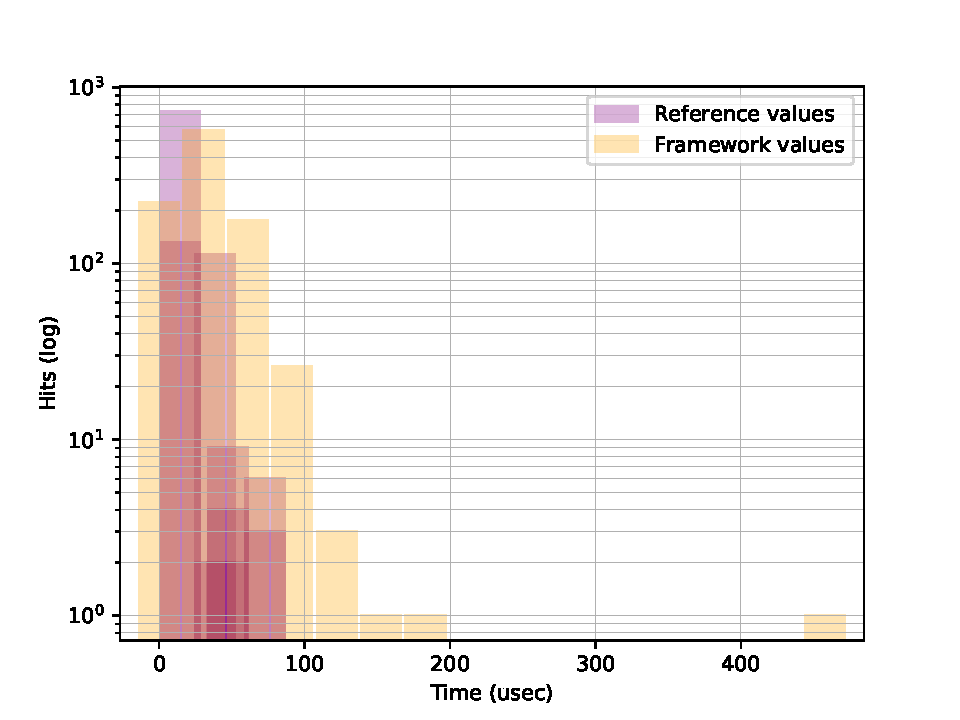
\includegraphics[scale=.4]{assets/comparison-extension-framework-contiki-remote.pdf}
%       \caption{Extension framework evaluation with Contiki on RE-Mote\label{fig:comparison-extension-framework-contiki-remote}}
%   \end{minipage}\hfill
%   \begin{minipage}{.45\textwidth}        
%       \centering
%       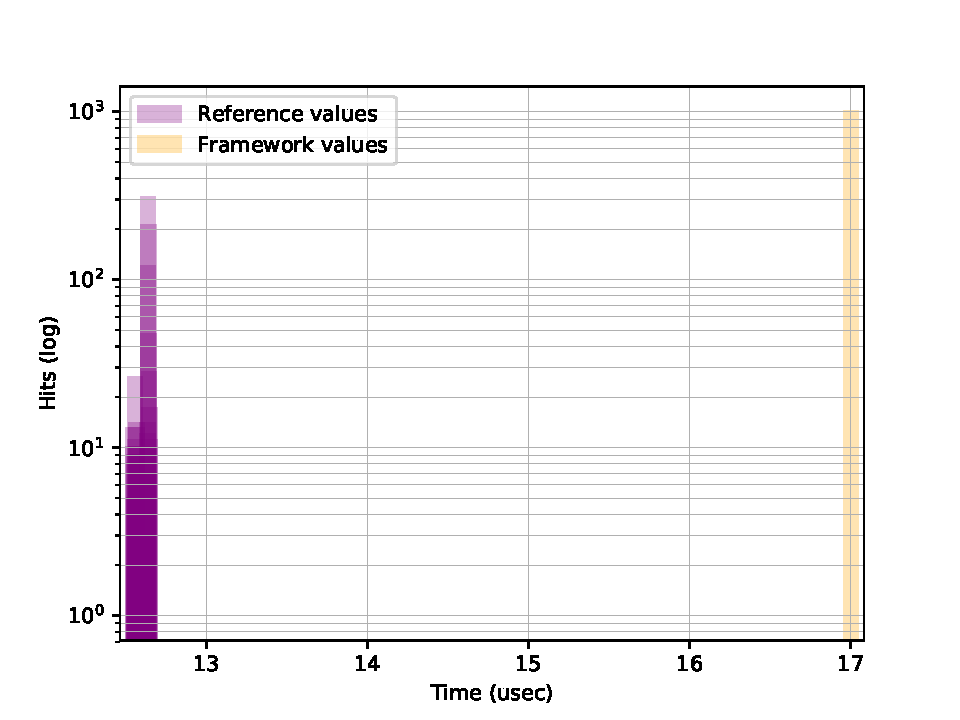
\includegraphics[scale=.4]{assets/comparison-extension-framework-riot-remote.pdf}
%       \caption{Extension framework evaluation with RIOT on RE-Mote\label{fig:comparison-extension-framework-riot-remote}}
%   \end{minipage}
% \end{figure}

% \begin{figure}[!ht]
%   \begin{minipage}{.45\textwidth}
%       \centering
%       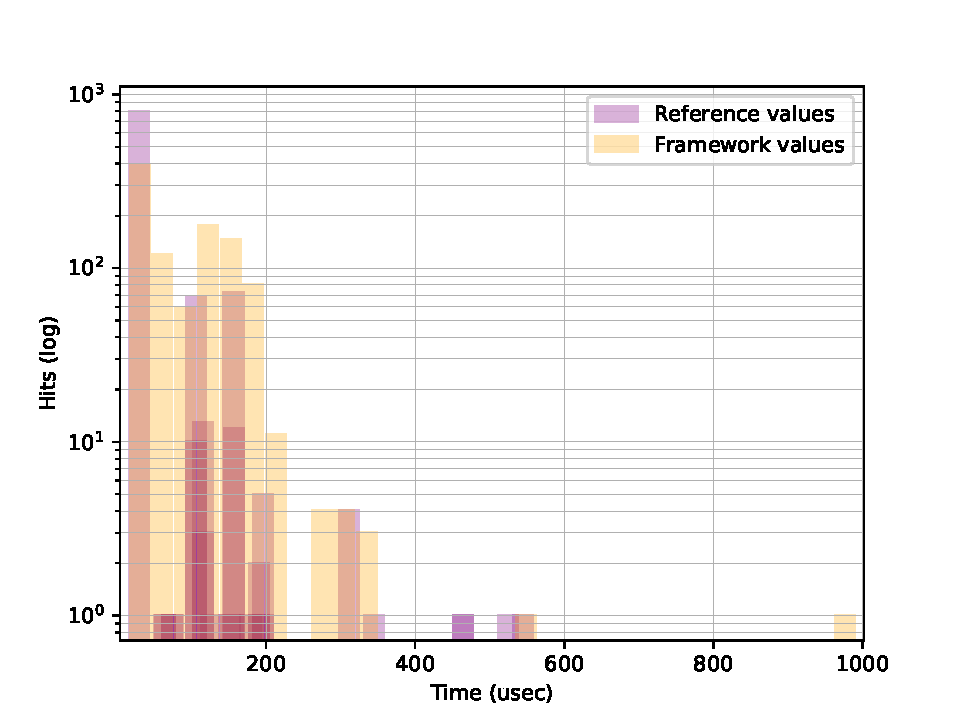
\includegraphics[scale=.4]{assets/comparison-extension-framework-contiki-z1.pdf}
%       \caption{Extension framework evaluation with Contiki on Z1\label{fig:comparison-extension-framework-contiki-z1}}
%   \end{minipage}\hfill
%   \begin{minipage}{.45\textwidth}        
%       \centering
%       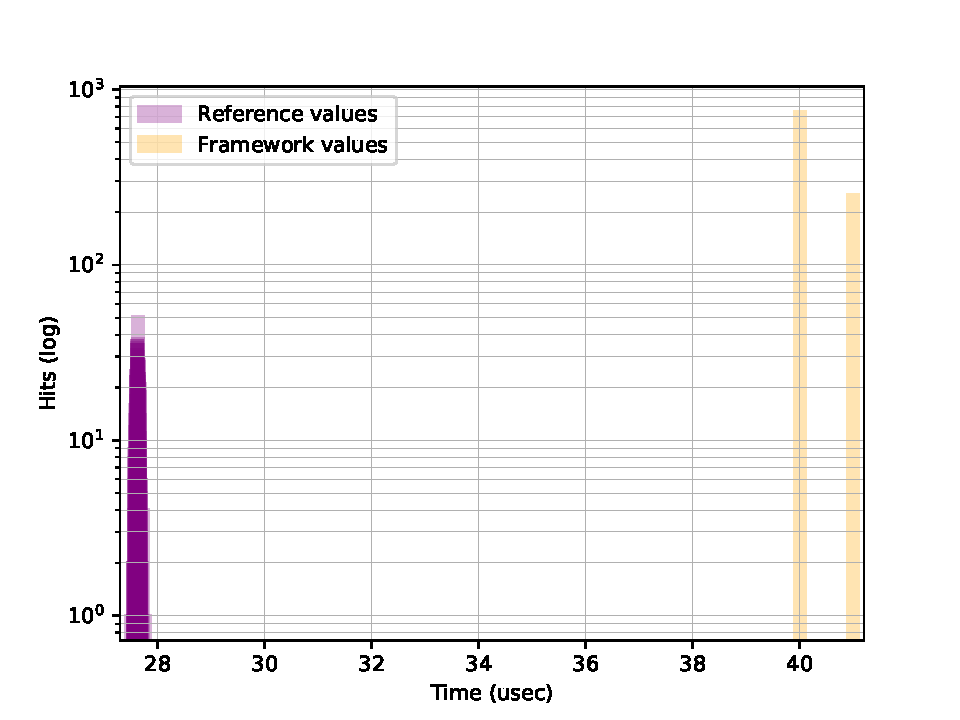
\includegraphics[scale=.4]{assets/comparison-extension-framework-riot-z1.pdf}
%       \caption{Extension framework evaluation with RIOT on Z1\label{fig:comparison-extension-framework-riot-z1}}
%   \end{minipage}
% \end{figure}

% \subsubsection{Limitation of the framework}
% As the results show, our extension framework is not able to compute the context switching time of our simple application.
% The devices do not have enough precision with their real-time clock.

\subsection{Devices framework measurement}

Generally, the measurements made with the devices framework are more accurate than the one made with the extension framework.

\subsubsection{RE-Mote measurements}
On the RE-Mote board, the devices framework outputs an average context switching time of $19.0329\mu s$ on Contiki and $13.9829 \mu s$ on RIOT OS.
The table \ref{tab:devices-framework-remote} shows the measurement for Contiki and RIOT OS for the RE-Mote board.

\begin{table}[!ht]
  \centering
  \begin{tabular}{l|c|c}
                & Contiki  & RIOT \\ \hline
  Mean ($\mu$s) & 19.0329  & 12.9823 \\
  Min  ($\mu$s) & 14.9375  & 12.9375 \\
  Max  ($\mu$s) & 91.75    & 13.0156
  \end{tabular}
  \caption{devices framework measurements for Contiki and RIOT on the RE-Mote board}
  \label{tab:devices-framework-remote}
  \end{table}

For Contiki, the majority of the values were around $14\mu s$ but some of them were above $40\mu s$.
For RIOT, the measurement were either around $13 \mu s$ or around $14.89 \mu s$.
The figure \ref{fig:devices-framework-contiki-remote} and the figure \ref{fig:devices-framework-riot-remote} show those distributions.

\begin{figure}[!ht]
%   \begin{minipage}{.45\textwidth}
      \centering
      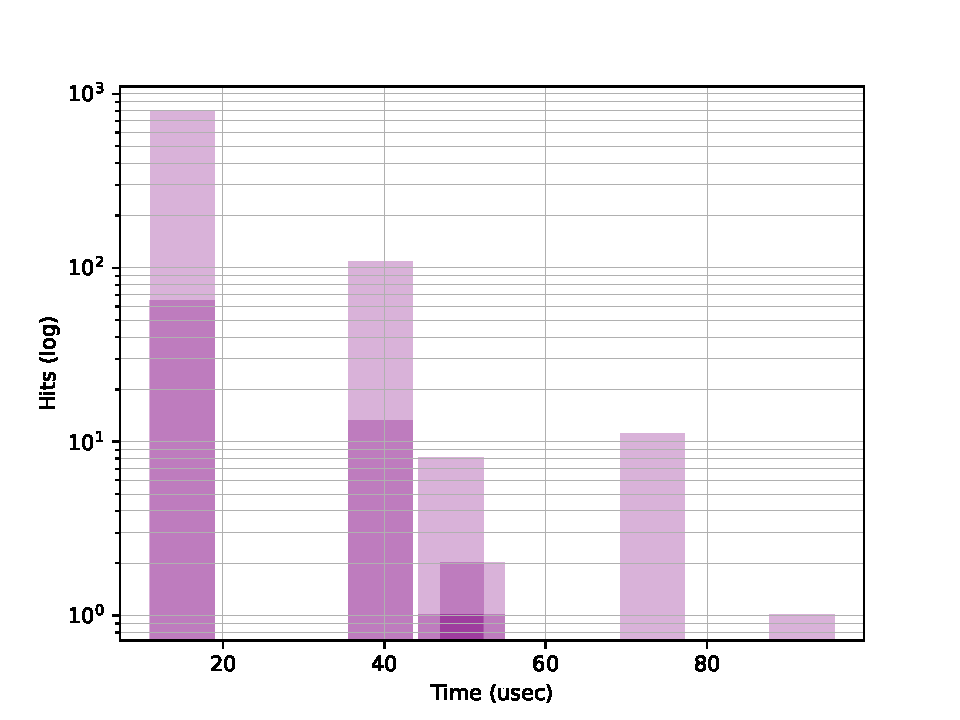
\includegraphics[scale=.8]{assets/devices-framework-contiki-remote.pdf}
      \caption{Devices framework distribution with Contiki on RE-Mote\label{fig:devices-framework-contiki-remote}}
%   \end{minipage}\hfill
%   \begin{minipage}{.45\textwidth}        
      \centering
      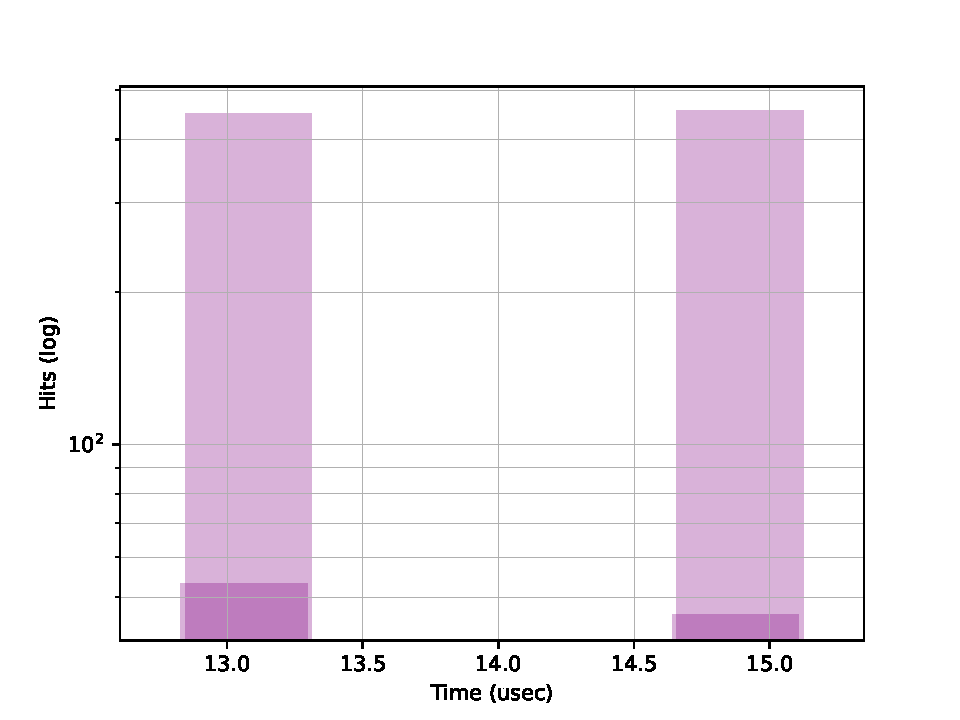
\includegraphics[scale=.8]{assets/devices-framework-riot-remote.pdf}
      \caption{Devices framework distribution with RIOT on RE-Mote\label{fig:devices-framework-riot-remote}}
%   \end{minipage}
\end{figure}

By comparing the measurement with our reference value, the difference between the real context switching time and the context switching time measured by our devices frameowrk is $0.5279\mu s$ with Contiki and $1.3569\mu s$ with RIOT.

\subsubsection{Z1 measurements}
The devices framework found a context switching time of $54.99\mu s$ with Contiki and $30.6971\mu s$ with RIOT OS on the Z1 board.
The difference with the real context switching time is close to $0\mu s$ with Contiki but close to $3\mu s$ with RIOT OS.
The table \ref{tab:devices-framework-z1} shows the measurement for both Contiki and RIOT OS on the Z1 board.

\begin{table}[!ht]
  \centering
  \begin{tabular}{l|c|c}
                & Contiki  & RIOT OS \\ \hline
  Mean ($\mu$s) & 54.99    & 30.6971 \\
  Min  ($\mu$s) & 32.5625  & 30.5312 \\
  Max  ($\mu$s) & 314.5    & 30.8437
  \end{tabular}
  \caption{devices framework measurements for Contiki and RIOT on the Z1 board}
  \label{tab:devices-framework-z1}
  \end{table}

However, on Contiki the measured values are more scattered.
The minimum measured context switching time is $32.5625\mu s$ and the maximum one is $314.5\mu s$.
In the other hand, with RIOT, we have a nice distribution around $30.6971\mu s$.
The figure \ref{fig:devices-framework-contiki-z1} and the figure \ref{fig:devices-framework-riot-z1} show those distributions.

\begin{figure}[!ht]
%   \begin{minipage}{.45\textwidth}
      \centering
      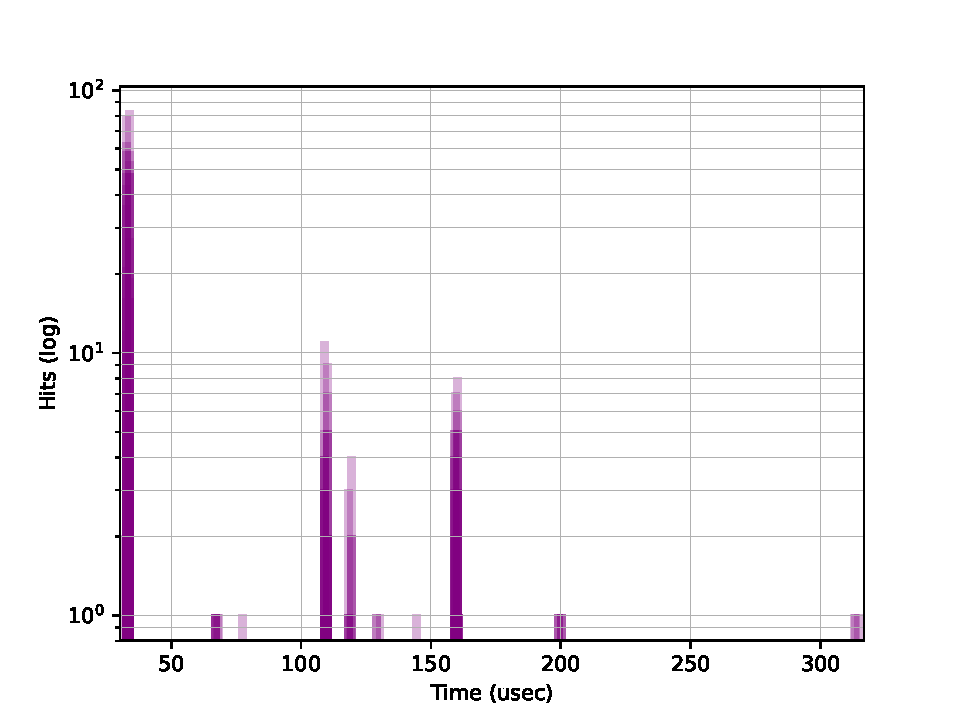
\includegraphics[scale=.8]{assets/devices-framework-contiki-z1.pdf}
      \caption{Devices framework distribution with Contiki on Z1\label{fig:devices-framework-contiki-z1}}
%   \end{minipage}\hfill
%   \begin{minipage}{.45\textwidth}        
      \centering
      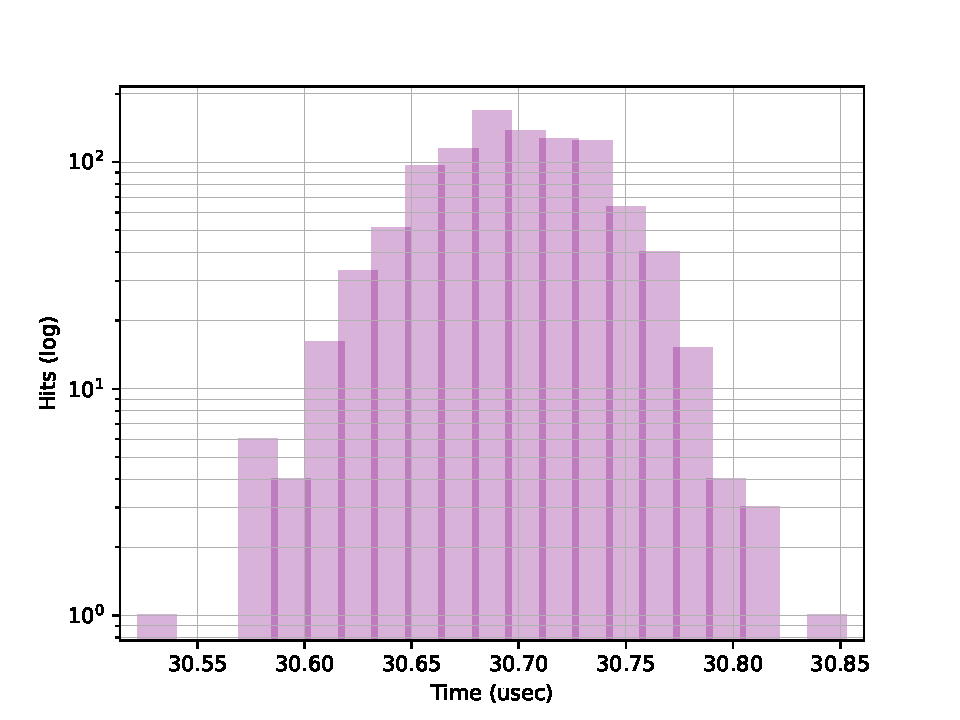
\includegraphics[scale=.8]{assets/devices-framework-riot-z1.pdf}
      \caption{Devices framework distribution with RIOT on Z1\label{fig:devices-framework-riot-z1}}
%   \end{minipage}
\end{figure}

% \subsection{Discussion}

% \subsubsection{Comparisons}

% \begin{figure}[!ht]
%   \begin{minipage}{.45\textwidth}
%       \centering
%       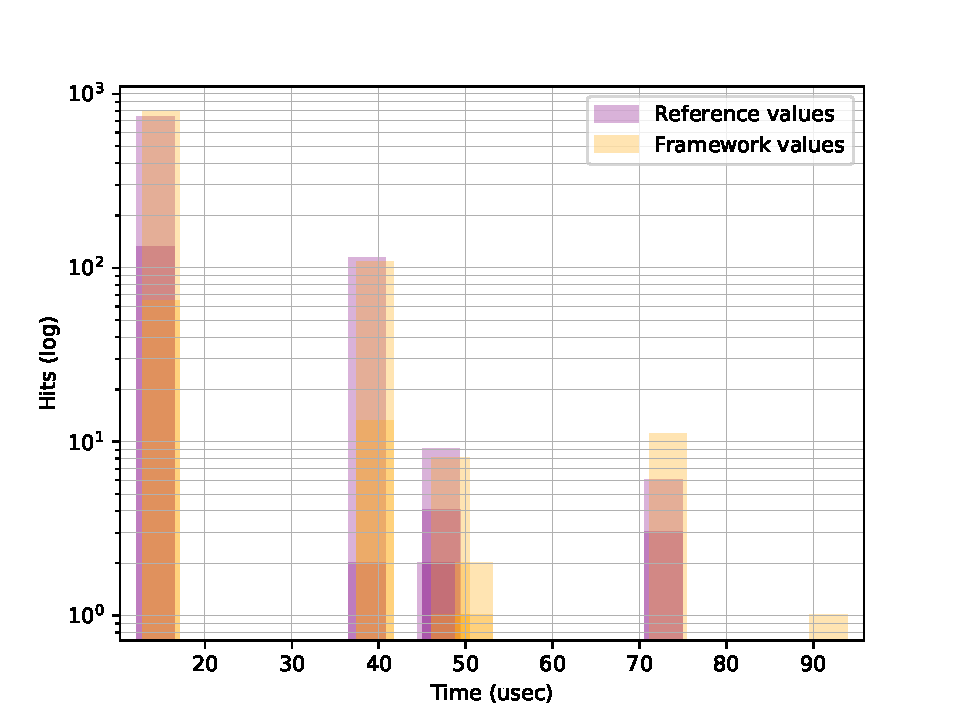
\includegraphics[scale=.4]{assets/comparison-devices-framework-contiki-remote.pdf}
%       \caption{Devices framework evaluation with Contiki on RE-Mote\label{fig:comparison-devices-framework-contiki-remote}}
%   \end{minipage}\hfill
%   \begin{minipage}{.45\textwidth}        
%       \centering
%       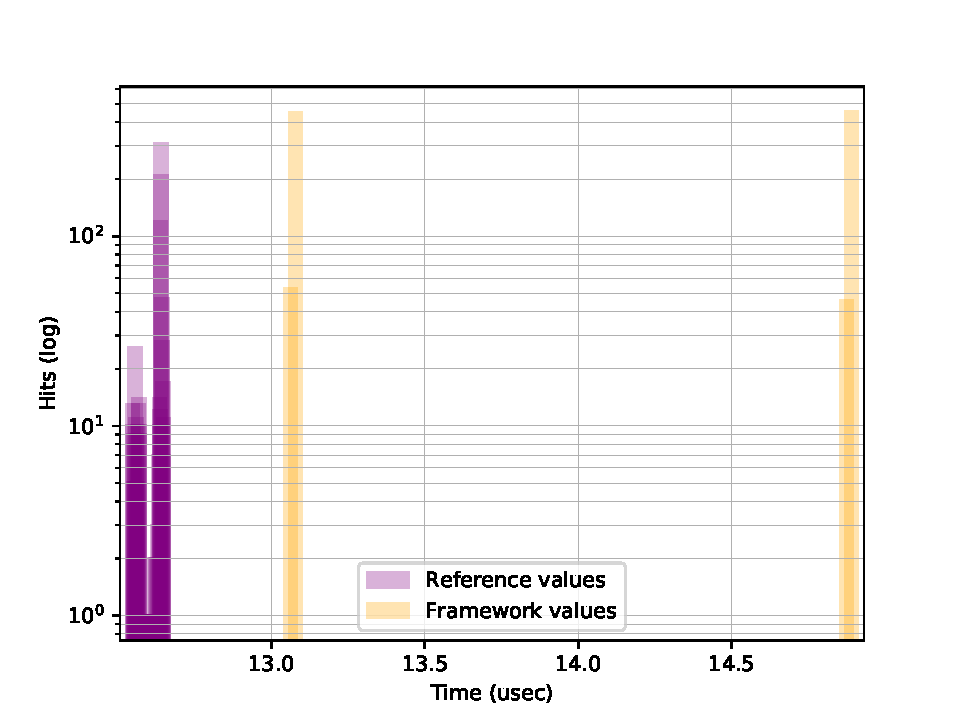
\includegraphics[scale=.4]{assets/comparison-devices-framework-riot-remote.pdf}
%       \caption{Devices framework evaluation with RIOT on RE-Mote\label{fig:comparison-devices-framework-riot-remote}}
%   \end{minipage}
% \end{figure}

% \begin{figure}[!ht]
%   \begin{minipage}{.45\textwidth}
%       \centering
%       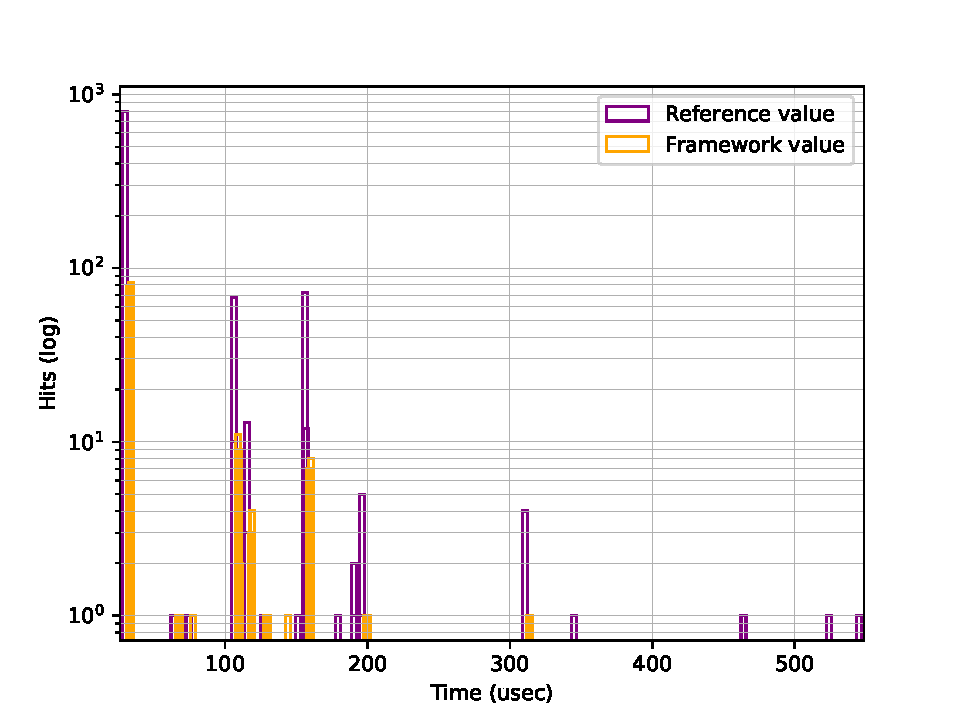
\includegraphics[scale=.4]{assets/comparison-devices-framework-contiki-z1.pdf}
%       \caption{Devices framework evaluation with Contiki on Z1\label{fig:comparison-devices-framework-contiki-z1}}
%   \end{minipage}\hfill
%   \begin{minipage}{.45\textwidth}        
%       \centering
%       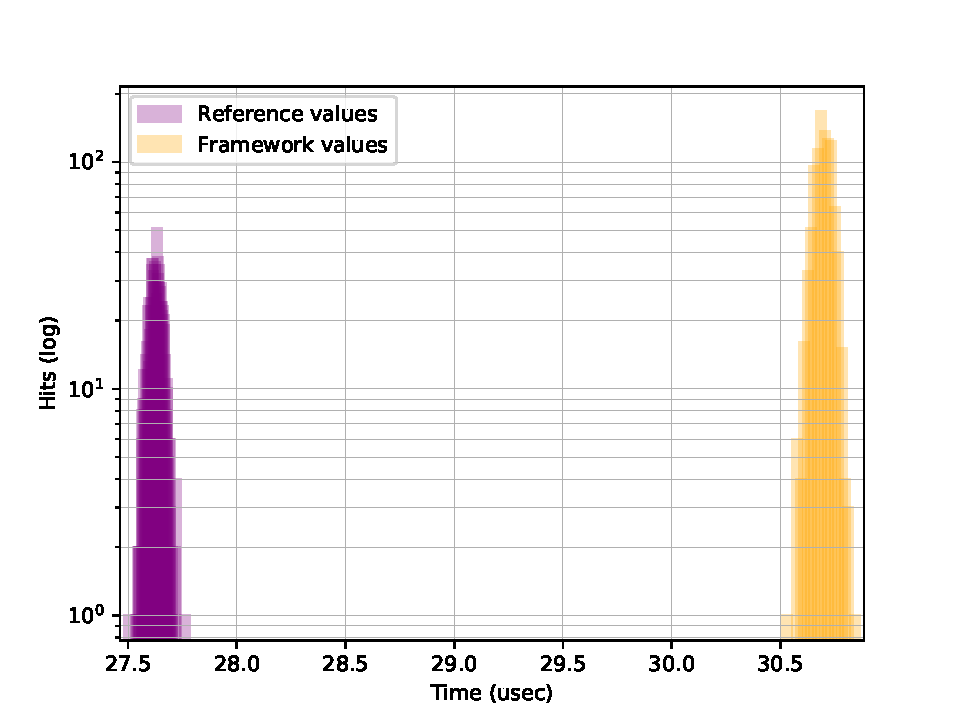
\includegraphics[scale=.4]{assets/comparison-devices-framework-riot-z1.pdf}
%       \caption{Devices framework evaluation with RIOT on Z1\label{fig:comparison-devices-framework-riot-z1}}
%   \end{minipage}
% \end{figure}